\documentclass{article}
\usepackage{graphicx}
\usepackage[dutch]{babel}
\usepackage{amssymb}      %for use of liveness operator

\begin{document}
\sffamily
\begin{titlepage}
  \centering
    \vfill
    {\bfseries\Huge
      Verslag Tinlab Advanced Algorithms \\
        \vskip2cm
      }
      {\bfseries\Large
        Noëlle Clement\\
      }
      {
        \bfseries\normalsize
        0935050\\
        \vskip1cm
        \today\\
    }
    \vfill
    
\includegraphics[width=4cm]{../resources/logohr.png} % also works with logo.pdf
    \vfill
    \vfill
\end{titlepage}

\newpage
\tableofcontents

\newpage
\section{Inleiding}
  Dit verslag is samengesteld als naslagwerk van de theorie uit de Tinlab 'Advanced Algorithms' gegeven door Wessel Oele en Elvira van der Ven. Binnen dit vak hebben we geleerd over softwareverificatie en wat daar bij komt kijken. Hierdoor komen ook onderwerpen zoals requirements, transition diagrams en temporele logica aan bod. Voor meer informatie over het praktische gedeelte van dit vak verwijs ik graag door naar het projectverslag dat door Tommie Terhoeve en mij (Noëlle Clement) is samengesteld.

\newpage
\section{Requirements}
  %uitleg requirements
  %requirements vs specifications
  %belang > correct opstellen belangrijk (heeft impact, safety-critical bron)
  %hoe opgesteld? (tips, bijv sos bron)
  %vier variabelen model?

  %mode confusion
  %automatiseringsparadox

  %rampen

  \subsection{Requirements}
    \textit{In dit hoofdstuk gaan we dieper in op requirements - eisen die gesteld worden aan systemen. Hierbij is het belangrijk om rekening te houden met de verscheidende meningen in het (wetenschappelijke) werkveld hierover. Onderstaande is dus een samenstelling van een gedeelte van deze meningen en visies.} \\\\
    Een systeem wordt gedefinieerd als twee of meer componenten die interactief samenwerken aan een gemeenschappelijk doel. Hierbij focussen we op ‘system engineering’ dat zich bezighoudt met het ontwikkelen van kunstmatige (door de mens gemaakte) systemen. Dit door de mens gecreëerde systeem wordt ontwikkeld om een gepland doel(einde) te behalen. Meestal bevat het systeem computersoftware en mensen die de hardware en software besturen om het vastgestelde doel van het systeem te behalen \cite{grady2010system}. \\\\
    Het systeem heeft interactie met de ‘systeemomgeving’ en zichzelf om de systeemfunctie of –doelstelling te behalen. De systeemomgeving bevat alles dat het systeem beïnvloed, naast het systeem zelf \cite{grady2010system}.\\\\
    ‘Systeem requirements’ zijn gedefinieerde attributen van het systeem, die worden vastgesteld voordat het systeem wordt ontworpen. Een ‘systeem requirements analyse’ wordt uitgevoerd om tot een reeks voorzieningen te komen, die ervoor gaan zorgen dat het systeem aan de systeem requirements zal voldoen. De analyse zet de klant/gebruiker behoeftes om in een ontwerp, zodat de ontwikkelaars van het systeem hiermee aan de slag kunnen \cite{grady2010system}. \\\\
    Het resultaat van de systeem requirements analyse is de 'requirements specification'. Waar een requirement 1 functie of kwaliteit van het systeem definieerd, is de requirement specification een collectie van alle requirements die in het design moeten terugkomen, en geverifieerd moeten worden \cite{hooks2015difference}.
    Atlee en Gannon geven de volgende definitie voor requirement specification: "De gedragsspecificatie van de systeemactiviteiten". Dit bevat vaak een reeks veiligheidsbeweringen die gehandhaafd moeten worden \cite{gannon1993state}. \\\\
    Hiernaast is er ook nog een verschil te definiëren tussen requirements specification en design specification. Requirements specification houdt zich bezig met de 'wat', de design specification met de 'hoe' \cite{hooks2015difference}. \\\\
    Maar waarom is het van belang om deze dingen zo duidelijk te definiëren? \\\\
    'Safety-critical' systemen, waarbij het van groot belang is dat de software in het systeem zich 'gedraagd’ als gewenst, vormen hiervoor een goed voorbeeld. Wassyng en Lawford leggen uit dat bij ‘safety-critical’ projecten, het ontwerp geverifieerd moet kunnen worden (vaak wiskundig tegen de requirements). Het ontwerp moet dan dus voldoende gedetaileerd zijn om een complete specificatie te hebben van het gedrag, zodat de code aan de hand hieraan kan worden ontwikkeld, getest en geverifieerd \cite{wassyng2006software}. \\\\
    Een ander voorbeeld van een systeem waarbij het duidelijke definiëren van groot belang is, is het System of Systems (SOS). Bij SOS's heeft men te maken met verschillende systemen die met elkaar samenwerken, waardoor het extra complex is. Door deze verhoogde complexiteit moet er dus ook extra goed gekeken worden naar hoe de kans op fouten in het systeem zoveel mogelijk kan worden verkleind. Hooks adviseert hierover ondere andere het volgende: "In product ontwikkeling is het essentieel om de 'scope' van het product vast te stellen, voordat de requirements worden opgesteld. [...] De scope bevat de behoefte(s), doeleind(en), en doelstelling(en)."  \cite{hooks2004sos}. \\


  \subsection{Specification}
    Om het allemaal nog wat ingewikkelder te maken, wordt het ook nog onderscheid gemaakt tussen requirements en specifications. Hierbij wordt iets anders bedoeld dan requirement specification en zijn specifications meer gelijk aan de design specifications die al eerder genoemd zijn. In systemen met een software component worden ze vaak ook wel 'software requirements' genoemd. \\\\
    Het bovenstaande klinkt wellicht al complex, maar er is veel onduidelijkheid over de definities van de termen. Wiegers en Joy geven dit ook al aan in hun boek, en hanteren de volgende definitie: "[Software] requirements zijn specificaties van wat geïmplementeerd zou moeten worden. Ze omschrijven hoe het systeem zich zou moeten gedragen, of een systeemeigenschap of attribuut. \cite{wiegers2013software}". \\\\
    Om wat duidelijkheid te creëeren is er bijvoorbeeld het 'four-variable model' ontwikkeld, zoals te zien in figuur~\ref{fig:fourvariablemodel}. Al zijn er velen die verbeteringen hebben voorgesteld aan het model, kan het zeker een goed overzicht geven. \\

    \begin{figure}[h]
      \centering
      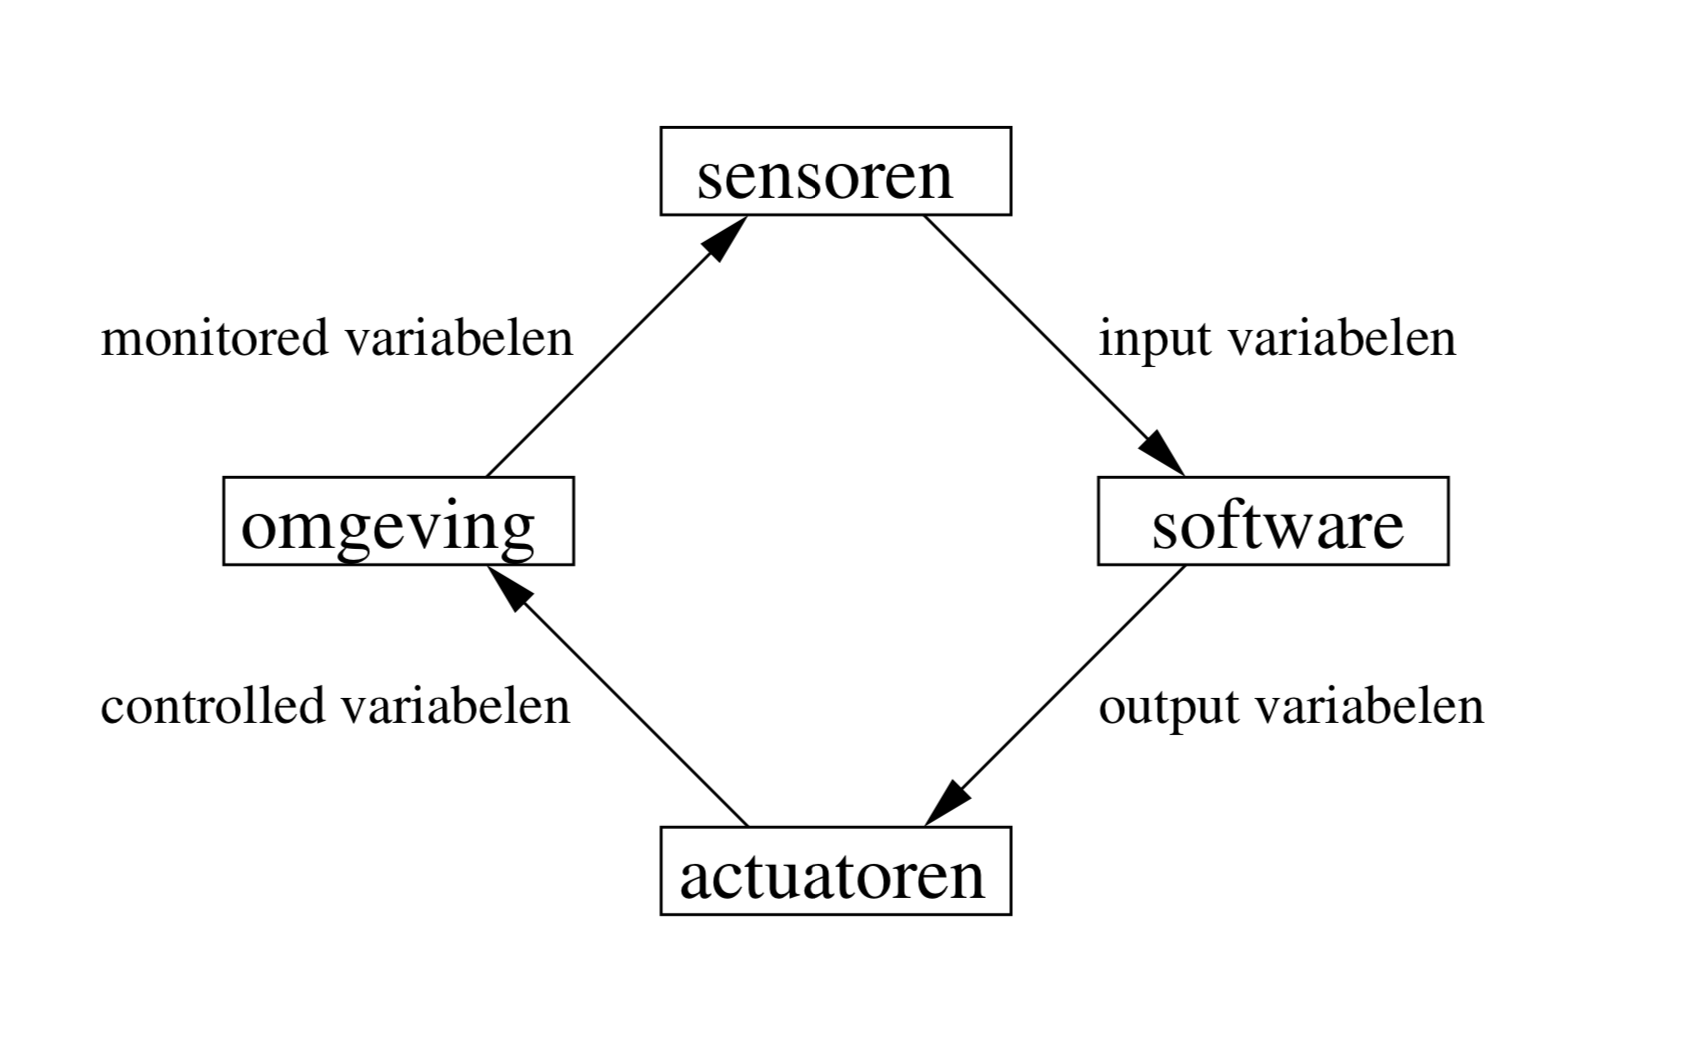
\includegraphics[scale=0.35]{../resources/fourvariablemodel}
      \caption{Four-variable model van Parnas en Madey (afbeelding van Wessel Oele)}
      \label{fig:fourvariablemodel}
    \end{figure}

    De variabelen hebben de volgende betekenissen \cite{miller2001extending}:
    \begin{itemize}
      \item Monitored variabelen komen uit de omgeving die het systeem observeert en op reageert.
      \item Controlled variabelen zijn in de omgeving die het systeem moet aansturen en/of beïnvloeden.
      \item Input variabelen laten de softare de monitored variabelen waarnemen.
      \item Output variabelen laten de software de controlled variabelen aanpassen.
    \end{itemize}

  \subsection{Mode confusion}
    Een probleem dat voor kan komen bij incorrect werkende systemen is mode confusion. Een mode is een waarde in een systeem dat invloed heeft op de veranderingen in het systeem. Onze huidige systemen hebben steeds meer modi, of 'states', en een verwarring in de huidige staat van een systeem kan tot grote problemen leiden. Mode confusion ontstaat wanneer de gebruiker van het systeem denkt dat het systeem zich in een andere staat bevindt dan waarin het zich werkelijk bevindt \cite{leveson1997analyzing}. \\\\
    Leveson et al beschrijven de volgende mogelijke soorten mode confusion \cite{leveson1997analyzing}:
    \begin{itemize}
      \item Interface modus errors: gebruiker denkt andere soort input te geven, dan welke het systeem 'verwacht'
      \item Onconsistent gedrag van het (geautomatiseerde) systeem
      \item Interne (indirecte) verandering van modus, zonder dat hier expliciete instructies voor gegeven zijn door de gebruiker
      \item Autorisatie limieten voor de gebruiker (waar wellicht wel toegang nodig is in noodgevallen)
      \item Onbedoelde bijeffecten
      \item Te weinig feedback vanuit het systeem naar de gebruiker
    \end{itemize}


  \subsection{Rampen analyse}
    Wat is er in het verleden fout gegaan in systemen, en waardoor werden deze fouten veroorzaakt?

    \subsubsection{Therac-25}
      Tussen 1985 en 1987 zijn er 6 incidenten van overbestraling geweest bij het gebruik van het Therac-25 bestralings apparaat. Hierbij zijn 3 patiënten zwaar gewond geraakt, en 3 patiënten overleden \cite{porrello2012death}. \\\\
      Uit onderzoek is gebleken dat de incidenten zijn ontstaan door problemen in het systeem. Het systeem gaf een errormelding aan de gebruiker, die deze kon omzeilen door het weg te klikken. Echter voerde het systeem dan nog steeds een (incorrecte) bestraling uit, wat ook tot mode confusion heeft geleid. Daarnaast zijn er ook verschillende besluiten genomen tijdens de ontwikkeling van het systeem, die tot verlaagde veiligheid hebben geleid, omdat de ontwikkelaar (onterecht) erg hoog vertrouwen had in het correct werken van het systeem \cite{bozdagtherac}. Er lijkt hier een probleem te zijn onstaan bij de output variabelen en controlled variabelen.

    \subsubsection{Vlucht 1951}
      Op 25 februari 2009 is vlucht TK1951 neergestort in de buurt van Schiphol Airport, tijdens nadering. Hierbij kwamen 9 mensen om het leven, en zijn 86 mensen gewond geraakt \cite{onderzoeksraad2010turkish}. \\\\
      Uit onderzoek is gebleken dat de linker radiohoogtemeter van het vliegtuig niet correct werkte, en een foutieve hoogte heeft doorgegeven aan het automatische gaspedaal. In de reglementen staat er beschreven dat bij het incorrect werken van het radiohoogtemetersysteem bij de onderhoudscheck, de daaraan gekoppelde automatische piloot niet mag worden ingeschakeld. Echter is er onduidelijkheid of dit gedurende de vlucht ook het geval zal zijn, omdat er niet een duidelijke waarschuwing wordt gegeven tijdens de vlucht wanneer het radiohoogtemetersysteem niet correct werkt. Een bijkomend probleem was dat het linker radiohoogtemetersysteem de incorrect waarde als een correct waarnam, en dus niet het reservesysteem liet inschakelen \cite{onderzoeksraad2010turkish}. Er lijkt hier dus een probleem te zijn onstaan bij de monitored variabelen, en de output variabelen.




\newpage
\section{Modellen}
  Zoals we in het vorige hoofdstuk hebben gelezen, is het belangrijk dat er bevestigd wordt dat het systeem zich gedraagt zoals gewenst. Dit kan bijvoorbeeld worden gedaan door het verifiëren van een model van het systeem dat moet worden ontwikkeld. Het verifiëren wordt gedaan door met temporele logica de overeenkomsten te checken tussen de uitspraken die uit de requirements ontstaan en het model. \\\\
  Zo'n soort model kan bijvoorbeeld een state transition diagram zijn, waarin de mogelijke toestanden (states) van het systeem te zien zijn. Ook wordt hierin de relaties tussen verschillende toestanden getoond.

  \subsection{Soorten modellen}
    Er zijn vele soorten state transition modellen, zoals:
    \begin{itemize}
      \item state transition diagrams
      \item labeled state transition diagrams
      \item timed state transition diagrams
      \item labeled timed state transition diagrams
      \item input-output state transition diagrams
      \item input enabled input-output state transition diagrams
      \item Kripke structuren
    \end{itemize}
    In de theorie in dit verslag zullen we focussen op Kripke structuren. Voor het praktische deel, het modelleren en verifiëren, gebruiken we een applicatie genaamd Uppaal, welke met labeled timed state transition diagrams werkt.

  \subsection{De Kripke structuur}
    De Kripke structuur is één van de soorten state transition modellen. Het differentieert zich van de andere soorten door de regels die gesteld zijn. Voordat we specifiek ingaan op deze regels worden 'states', 'transitions' en 'labels' uitgelegd. \\\\
    Men kan een 'werkend' systeem modelleren door middel van het doorlopen van een aantal states via transities.

    \subsubsection{States}
      Een 'state' is een beschrijving van het systeem gedurende een bepaald tijdsinterval. Het bevat de waarden van alle variabelen van het systeem gedurende dit tijdsinterval. Een belangrijk aspect is dat het niet 1 moment in tijd is. Het is de 'toestand' van het systeem in een periode, waarbij in die gehele periode het systeem zich in die staat bevindt, en dus alle variabelen hetzelfde blijven. Alle states in het model worden de 'states verzameling' genoemd.\\\\
      De beginstate bij het in werking zetten van het systeem heet de 'initial state'. In theorie zijn er verschillende mogelijke versies van die state, waardoor er over een initial states verzameling wordt gesproken. In de praktijk zien we echter dat het doorgaans maar één is. De initial states maken ook deel uit van de states verzameling. De initial states verzameling is dus een deelverzameling van de states verzameling.

    \subsubsection{Transitie}
      Wanneer het systeem een overgang maakt van ene state naar de andere, heet dit een transitie.\\\\
      Een belangrijke eis aan de modellen die wij gaan creëeren, is dat ze 'reactief' zijn. Dit houdt in dat alle states een uitgaande transitie hebben. Hierdoor kan er op dit vlak dus geen doodlopende weg ontstaan. Alle transitierelaties in onze modellen zijn dus 'totaal'.

    \subsubsection{Labels}
      Om uitspraken te kunnen doen over het gemodelleerde systeem wordt er gebruik gemaakt van een verzameling atomaire proposties (AP). AP's zijn proposities die niet verder op te delen zijn in kleinere of kortere proposities. Deze AP kun je toewijzen aan een state. We gaan hier op het moment niet verder op in, maar dit zal later in het verslag opnieuw aan bod komen.\\\\

    \subsubsection{4-tuple M}
      Als we alle onderdelen van een Kripke Structuur combineren tot een formule, komen we tot het volgende (de 4-tuple M):\\\\
      $ M = (S, S_0, R, L) $:\\\\
      $M$ = model \\
      $S$ = states verzameling \\
      $S_0 \subseteq S$ = initial states verzameling \\
      $R \subseteq S$ x $S$ = de transitierelatie \\
      $L: s \rightarrow 2^AP$ = labels (voor AP's per state)


  \subsection{Tijd}
    In een Kripke Structuur wordt er in principe geen gebruik gemaakt van tijd. Echter maakt Uppaal wel gebruik van diagrammen waar hier wel rekening mee wordt gehouden. \\\\
    Tijd wordt in Uppaal beschouwd als een continu verschijnsel, en wordt bijgehouden met klokken. De klokwaarden kunnen worden uitgelezen en bijvoorbeeld worden gebruikt voor invarianten en guards. \\\\
    Belangrijk hierbij is dat de tijd alleen in states verstrijkt, niet in de transities. Daarnaast wordt de klok gereset naar 0 bij het starten van het systeem. Ook spreken we van tijdseenheden, niet van (milli)seconden of minuten o.i.d.

    \subsubsection{Invarianten en Guards}
      Om condities aan de Kripke Structuur toe te voegen kunnen guards en invarianten gebruikt worden. In Uppaal kan het ook gebruikt worden om een transitie n.a.v. de tijd te forceren.

      \paragraph{Invariant}
        Een invariant is een conditie die altijd geldt wanneer het systeem zich in die state bevindt. Het kan daardoor gebruikt worden voor bijvoorbeeld voorkomen dat het systeem zich te vroeg in de staat bevindt. Ook kan het gebruikt worden om ervoor te zorgen dat het systeem op het goede moment uit de state 'verplaatst'.

      \paragraph{Guard}
        Een guard is een conditie die geldt in een transitie. De transitie kan daardoor alleen genomen worden wanneer het er aan voldoet.


    \subsubsection{Problemen bij gebruik van tijd}
      Het gebruik van tijd in je modellen heeft echter ook implicaties. Er moet rekening worden gehouden met problemen die kunnen ontstaan.

      \paragraph{Zeno gedrag}
        Wanneer er geen controle is op hoeveel handelingen worden uitgevoerd in een tijdseenheid, kan zeno gedrag voorkomen. Hierbij kunnen er oneindig veel handelingen verricht worden in een eindige hoeveelheid tijd. \\\\
        Een voorbeeld hiervan is te zien in figuur~\ref{fig:zenogedrag}. Aan de linker kant is te zien dat een invariant vereist dat er alleen toegang tot de state is wanneer de klok (x) kleiner of gelijk is aan 1. Hierbij is belangrijk te herinneren dat tijd niet verstrijkt in de transitie, en het is geen gegeven dat wanneer het systeem de transitie doorgaat dat de klok van 0 naar 1 gaat. Hierdoor weten we dus niet hoe vaak het systeem die transitie door gaat in die ene tijdseenheid. \\\\
        Een mogelijke oplossing hiervoor is het gebruik van guards (groen) en updates (blauw). Door via een guard de conditie op te leggen dat het alleen de transitie in mag wanneer de klok hoger of gelijk is dan 1, zorg je ervoor dat het duidelijker is wanneer de transitie genomen wordt. Daarnaast wordt de klok weer op 0 gezet, zodat er opnieuw correct gebruik kan worden gemaakt van de guard.

        \begin{figure}
          \centering
          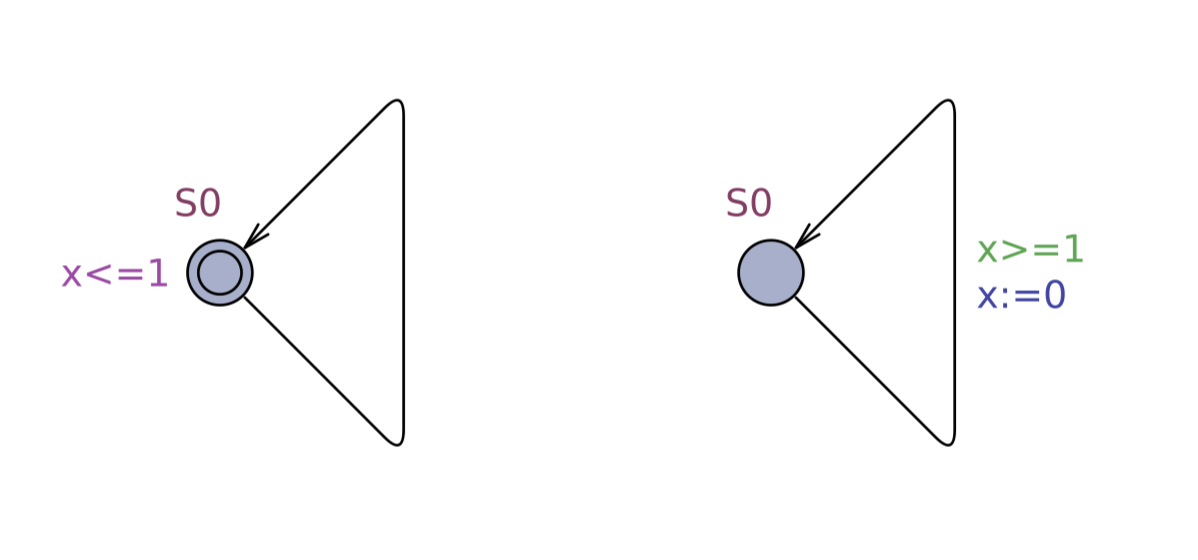
\includegraphics[scale=0.5]{../resources/zenogedrag}
          \caption{Zeno gedrag}
          \label{fig:zenogedrag}
        \end{figure}

      \paragraph{Deadlock}
        Wanneer processen oneindig lang op elkaar wachten in een besturingssysteem, wordt dit deadlock genoemd. In een model kan dit voorkomen wanneer een combinatie van invarianten en guards het verstrijken van tijd verhindert.
        %TODO eigen model die het duidelijk toont?

      \paragraph{Realisme van het model}
        Een transitie mag geen tijd kosten. Wanneer een systeem gemodelleerd wordt met een bewegend component, zouden in theorie oneindig veel states tijdens die beweging moeten worden gebruikt. Het modelleren van bewegende componenten moet dus anders aangepakt worden. Bij een deur kan bijvoorbeeld gebruik gemaakt worden van de states 'open', 'openen', 'gesloten' en 'sluiten'.


  \subsection{Parallelle compositie}
    Het is mogelijk om meerdere Kripke structuren tot 1 te combineren met behulp van parallelle compositie. Het kan nut hebben om parallelle compositie toe te passen wanneer je zeker wilt zijn dat de verschillende gedeeltes van het systeem bepaalde handelingen hebben verricht voordat het verder gaat. Bijvoorbeeld: een systeem kan pas worden opgestart na het indrukken van een knop, nadat de temperatuur ook is gecheckt.\\\\
    In figuur~\ref{fig:parallellecompositie} is te zien hoe het S en T model gecombineerd worden tot 1. Hierin is te zien dat ze beiden andere variabelen gebruiken (waarschijnlijk andere klokken in dit geval) en dat S en T eerst allebei state '1' (bij S1T1) moeten bereiken voordat het systeem verder kan. \\\\
    Bij het gebruik van parallelle compositie ontstaat wel een verhoogde kans op deadlocks, zeker wanneer de te combineren structuren gebruik maken van dezelfde variabelen. Ook kan het een model erg complex maken, wat verdere nadelen heeft.
    \begin{figure}[h]
      \centering
      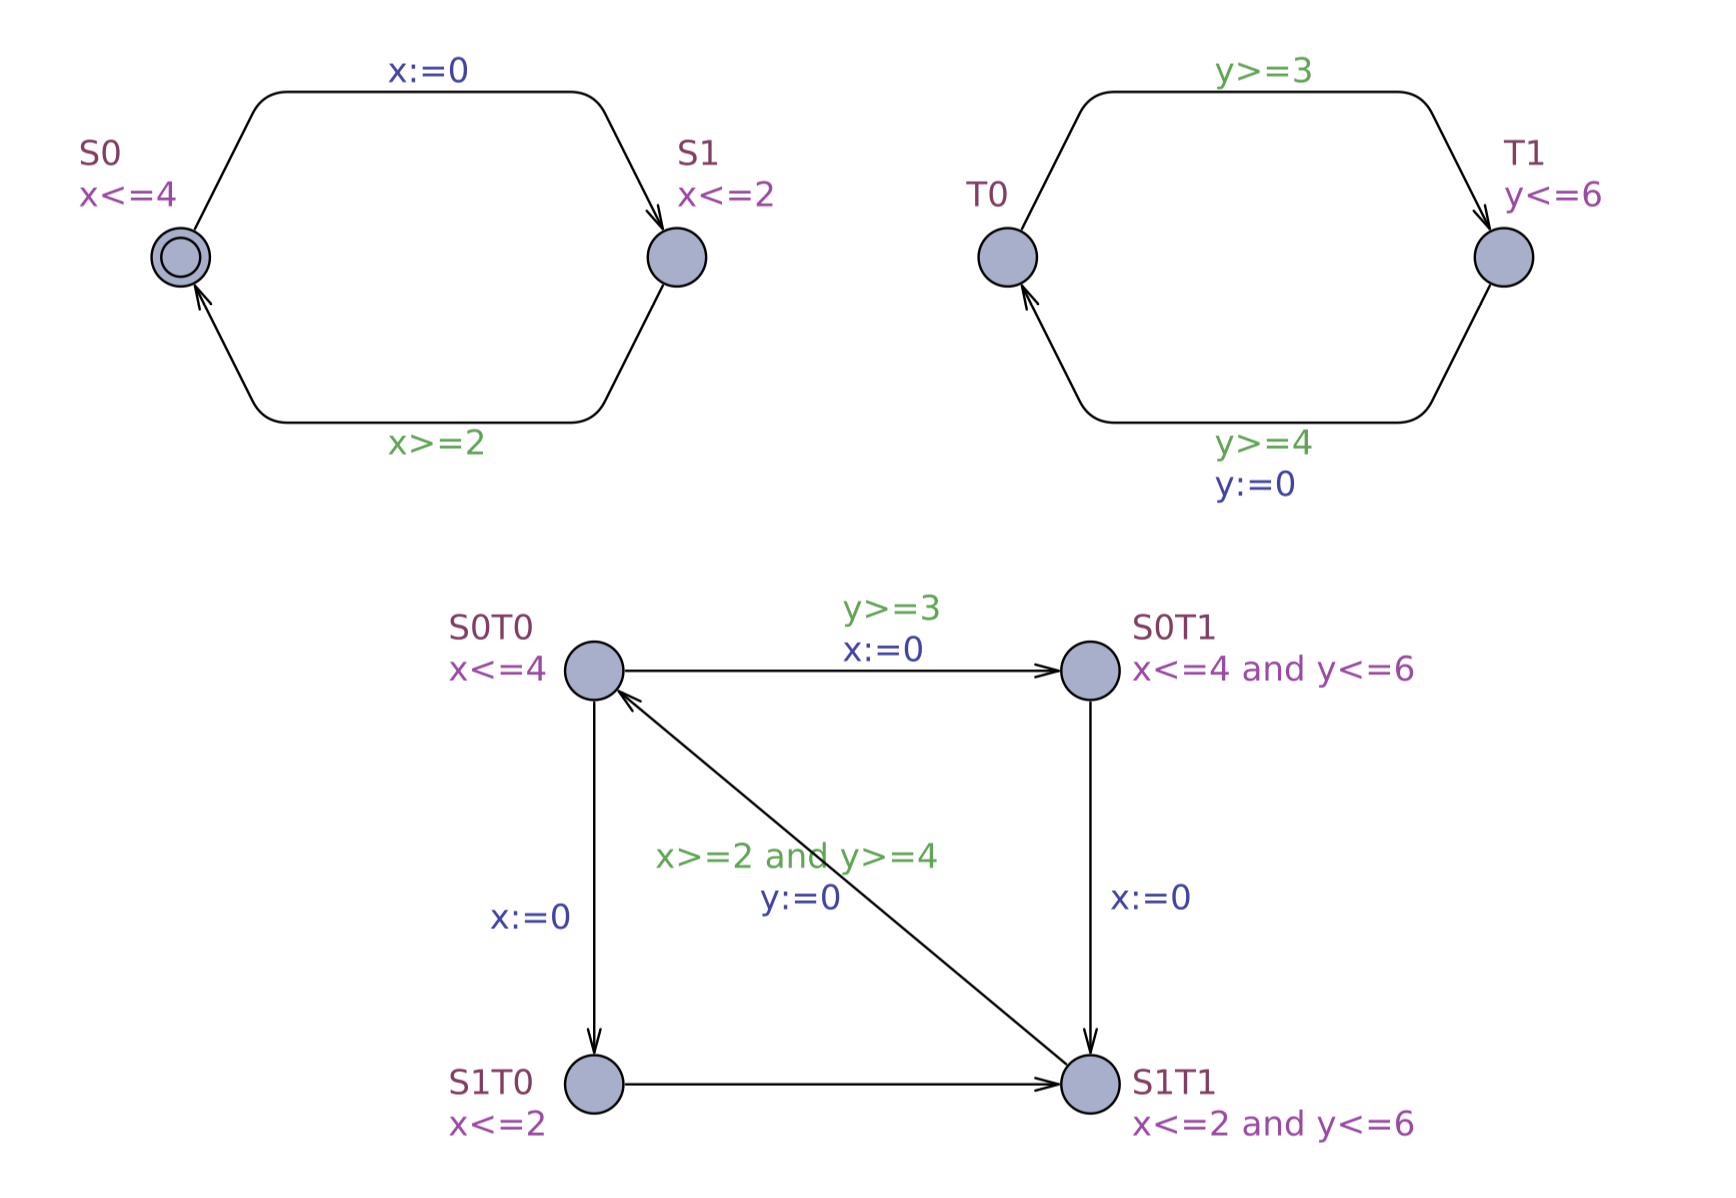
\includegraphics[scale=0.4]{../resources/parallellecompositie}
      \caption{Voorbeeld parallelle compositie}
      \label{fig:parallellecompositie}
    \end{figure}


\clearpage
\section{Logica}
% Propositional logic is the study of propositions, where a proposition is a statement that is either true or false. Propositional logic may be used to encode simple arguments that are expressed in natural language, and to determine their validity. The validity of an argument may be determined from truth tables, or using inference rules such as modus ponens to establish the conclusion via deductive steps. Predicate logic allows complex facts about the world to be represented, and new facts may be determined via deductive reasoning. Predicate calculus includes predicates, variables and quantifiers, and a predicate is a characteristic or property that the subject of a statement can have. bron: https://link.springer.com/chapter/10.1007/978-3-319-64021-1_6
% [Discrete Math 1] Introduction to Propositional Logic https://www.youtube.com/watch?v=itrXYg41-V0

  \subsection{Propositielogica}
    "In de propositielogica onderzoekt men het waarheidsgehalte van samengestelde uitspraken aan de hand van elementaire proposities en logische voegwoorden" \cite{oeleLogica}. Oftewel met propositielogica kunnen we wat zeggen over de uitspraken die gemaakt worden (in een zin), om hier meer (logische) structuur en inzicht in te brengen. \\\\
    Propositielogica is een tak van logica die werkt met proposities. Proposities zijn uitspraken die waar of onwaar zijn. Bijvoorbeeld: "Het regent" kan waar of onwaar zijn. \\\\ Doormiddel van logische operatoren kunnen er gecombineerde proposities gemaakt worden. De meest voorkomende logische operators zijn \cite{schaumsOutline}:
    \begin{itemize}
      \item $\wedge$ (AND): Conjunctie
      \item  $\vee$ (OR): Disjunctie
      \item  $\oplus$ (XOR) : Inclusieve disjunctie
      \item  $\lnot$ (NOT): Negatie, $\lnot$p betekent dat p niet waar is.
      \item  $\to$ : Implicatie, p $\to$ q betekent: Als p waar is dan is q ook waar.
    \end{itemize}

  \subsection{Predicatenlogica}
    %Is extension of proposite logic https://math.stackexchange.com/questions/9554/whats-the-difference-between-predicate-and-propositional-logic https://math.stackexchange.com/questions/2569217/is-predicate-logic-an-extension-of-propositional-logic
    %[Discrete Math 1] Predicate Logic and Negating Quantifiers https://www.youtube.com/watch?v=gyoqX0W-NH4&list=PLDDGPdw7e6Ag1EIznZ-m-qXu4XX3A0cIz&index=24&t=0s

    Predicatenlogica is een uitbreiding van de propositielogica. Wanneer men uitspraken wil doen over een verzameling (van 1 of meer), is dit niet mogelijk met propositielogica, omdat de waarheid van het enkele element al moest zijn vastgesteld. Om toch uitspraken te kunnen doen over verzamelingen, wordt predicatenlogica gebruikt \cite{schaumsOutline}. \\\\
    Net zoals in de propositielogica wordt er gebruik gemaakt van proposities en logische operators. In de predicatenlogica zijn er ook predicaten en kwantoren. Predicaten zeggen iets over de verzameling. Kwantoren geven aan over welk gedeelte van de verzameling de uitspraak wordt gedaan \cite{schaumsOutline}. \\\\
    Wanneer men de variabelen in een predicaat bindt aan een specifieke waarde, verkrijgen we een propositie. De elementen hebben dan een vaste waarheid gekregen, dus voldoen aan de propositielogica \cite{oeleLogica}. \\\\
    Predicatenlogica is van belang voor verificatie omdat we deze kunnen gebruiken om uitspraken te doen over verzamelingen. Zoals we eerder hebben gelezen, bestaan Kripke Structuren uit meerdere verzamelingen, waaronder de states-verzameling. Als je een uitspraak wilt doen over het gehele systeem (zoals 'nergens komt deadlock voor') zul je dus predicatenlogica gebruiken. \\\\\\\\
    Van groot belang hierin zijn kwantoren \cite{schaumsOutline}:
    \begin{center}
      \begin{tabular}{|ccc|}
        \hline
        uitspraak & symbolisch & naam \\
        \hline
        “voor alle x” & \forall~x & universele kwantor \\
        “er zijn x” & \exists~x & existentiële kwantor \\
        \hline
      \end{tabular}
    \end{center}

  \subsection{Dualiteiten}
    Dualiteiten zijn formules of relaties die uiteindelijk hetzelfde betekenen, in de logica een soort wiskundige synoniemen dus. Twee bekende voorbeelden in de propositielogica zijn de wetten van De Morgan. Voor twee proposities P en Q gelden de volgende wetten \cite{oeleLogica}:
    \begin{itemize}
      \item $\lnot$ (P$\wedge$Q) = ($\lnot$P $\vee$ $\lnot$Q)
      \item $\lnot$ (P$\vee$Q) = ($\lnot$P $\wedge$ $\lnot$Q)
    \end{itemize}


\newpage
\section{Computation Tree Logic}
  Een verdere uitbreiding op propositie- en predicatenlogica, is de temporele logica. Hierbij wordt het element 'tijd' bijgevoegd. Computation Tree Logic (CTL) is een vorm van temporele logica \cite{modelchecking}, en een subset hiervan wordt gebruikt voor het verifiëren van een Kripke structuur in Uppaal \cite{behrmann2006tutorial}.\\\\
  De vraag of een Kripke structuur een bepaalde in CTL geformuleerde eigenschap bezit kan middels een algoritme worden beantwoord. Hierbij worden op het achtergrond dualiteiten gebruikt om dit efficiënt af te handelen. Door dit alles is het volledig geautomatiseerd checken - verifiëren - van een (model van een) systeem mogelijk \cite{modelchecking}. Voorbeelden van CTL dualiteiten zijn:
  \begin{itemize}
    \item AX(f) = $\lnot$EX($\lnot$f)
    \item AG(f) = $\lnot$EF($\lnot$f)
  \end{itemize}
  CTL (met gebruik van kwantoren) maakt het mogelijk logische uitspraken te doen een Kripke structuur. Deze uitspraken kunnen bijvoorbeeld worden gedaan over of een state bereikt of verlaten kan worden, en via welke weg dit wordt gedaan. Hierbij is de computation tree van groot belang. De computation tree toont namelijk de mogelijke paden waar het systeem zich door kan verwerken \cite{modelchecking}.\\\\
  Om de uitspraken te kunnen formuleren, worden in CTL operatoren gebruikt die erg veel weg hebben van kwantoren. Hieronder meer over de meest gebruikte operatoren \cite{modelchecking}:

  \subsection{Operator: AG}
    \begin{itemize}
      \item Always - Globally
      \item in elk pad is deze uitspraak altijd waar
    \end{itemize}
    \begin{figure}[h]
      \centering
      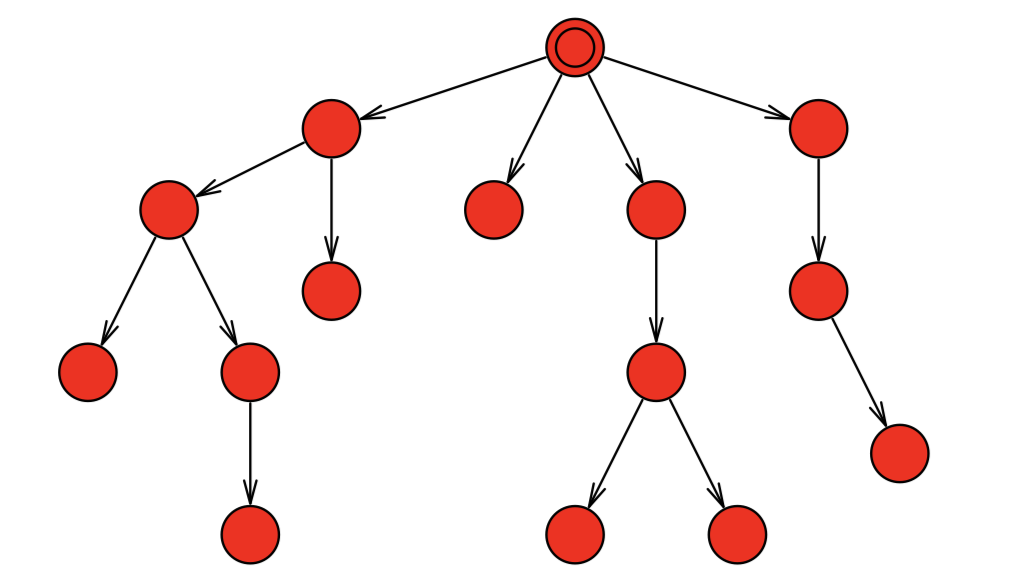
\includegraphics[scale=0.4]{../resources/AG}
      \caption{Voorbeeld computation tree: operator AG}
      \label{fig:ag}
    \end{figure}

  \subsection{Operator: EG}
    \begin{itemize}
      \item Exists - Globally
      \item In sommige paden is deze uitspraak altijd waar
    \end{itemize}
    \begin{figure}[h]
      \centering
      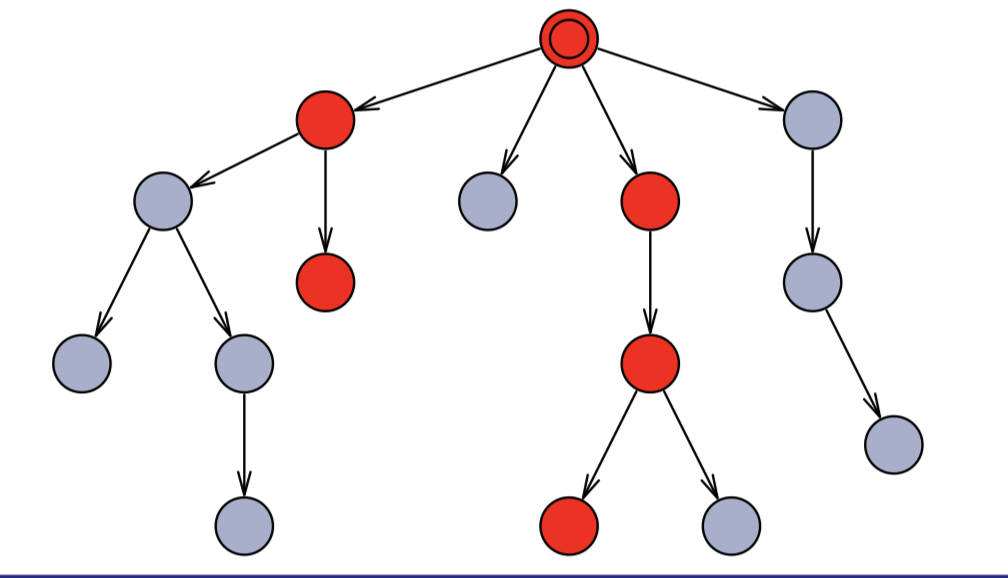
\includegraphics[scale=0.4]{../resources/EG}
      \caption{Voorbeeld computation tree: operator EG}
      \label{fig:eg}
    \end{figure}

  \subsection{Operator: AF}
    \begin{itemize}
      \item Always - Eventually
      \item In elk pad is deze uitspraak uiteindelijk waar
      \item Kan ook meerdere keren in 1 pad voorkomen
    \end{itemize}
    \begin{figure}[h]
      \centering
      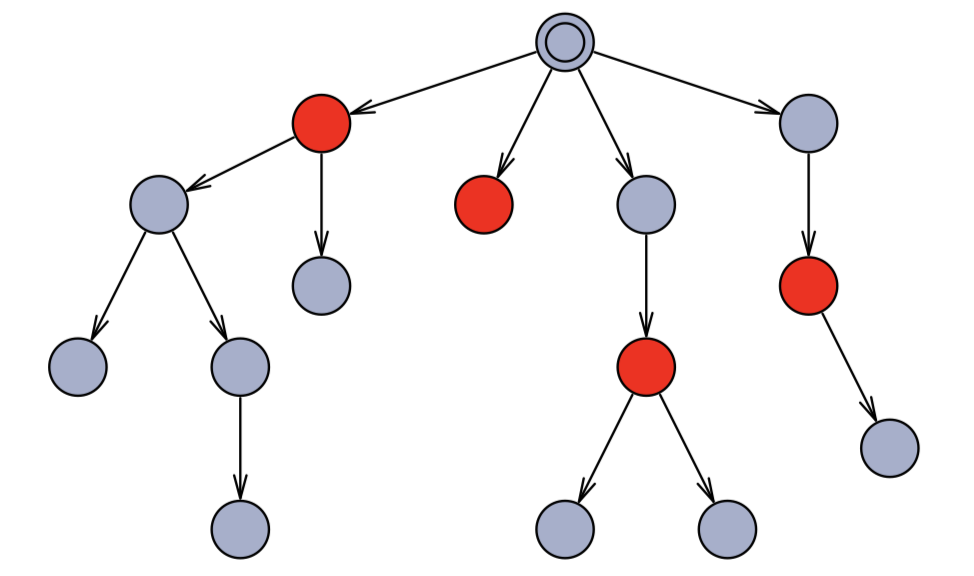
\includegraphics[scale=0.4]{../resources/AF}
      \caption{Voorbeeld computation tree: operator AF}
      \label{fig:af}
    \end{figure}


  \subsection{Operator: EF}
    \begin{itemize}
      \item Exists - Eventually
      \item In sommige paden is deze uitspraak uiteindelijk waar
      \item Kan ook meerdere keren in 1 pad voorkomen
    \end{itemize}
    \begin{figure}[h]
      \centering
      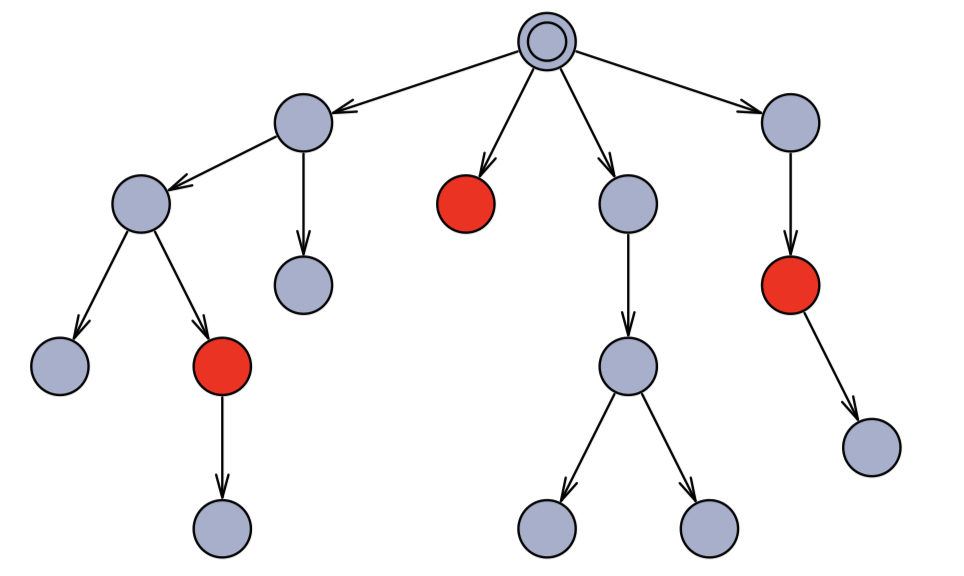
\includegraphics[scale=0.4]{../resources/EF}
      \caption{Voorbeeld computation tree: operator EF}
      \label{fig:ef}
    \end{figure}


  \subsection{Operator: AX}
    \begin{itemize}
      \item Always - Next
      \item In alle volgende states is deze uitspraak waar
      \item Wordt voornamelijk gebruikt voor uitspraken vanuit de initial state
    \end{itemize}
    \begin{figure}[h]
      \centering
      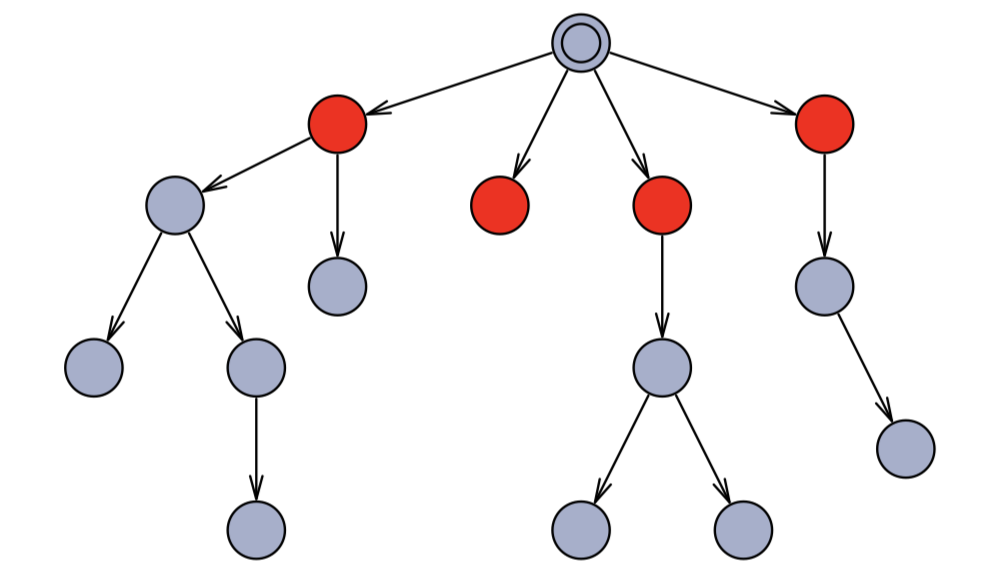
\includegraphics[scale=0.4]{../resources/AX}
      \caption{Voorbeeld computation tree: operator AX}
      \label{fig:AX}
    \end{figure}


  \subsection{Operator: EX}
    \begin{itemize}
      \item Exists - Next
      \item In sommige volgende states is deze uitspraak waar
      \item Wordt voornamelijk gebruikt voor uitspraken vanuit de initial state
    \end{itemize}
    \begin{figure}[h]
      \centering
      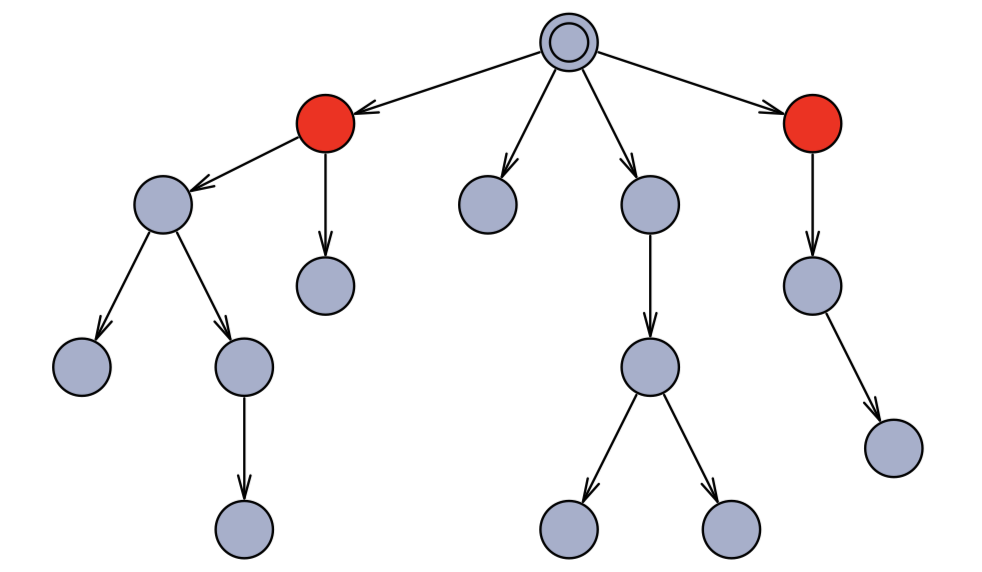
\includegraphics[scale=0.4]{../resources/EX}
      \caption{Voorbeeld computation tree: operator EX}
      \label{fig:ex}
    \end{figure}


  \subsection{Operator: p U q}
    \begin{itemize}
      \item 'p' Until 'q'
      \item Uitspraak 'p' is waar voor de states in het pad, totdat 'q' waar is
      \item Er is geen moment (en state) in de transitie van 'p' naar 'q' waarin beide uitspraken waar zijn
      \item 'q' blijft niet noodzakelijk waar na de transitie
      \item 'p U q' geldt ook als 'q' waar is (vanuit logica)
    \end{itemize}

      \subsubsection{A(p U q)}
        In elk pad geldt 'p U q'.
        \begin{figure}[h]
          \centering
          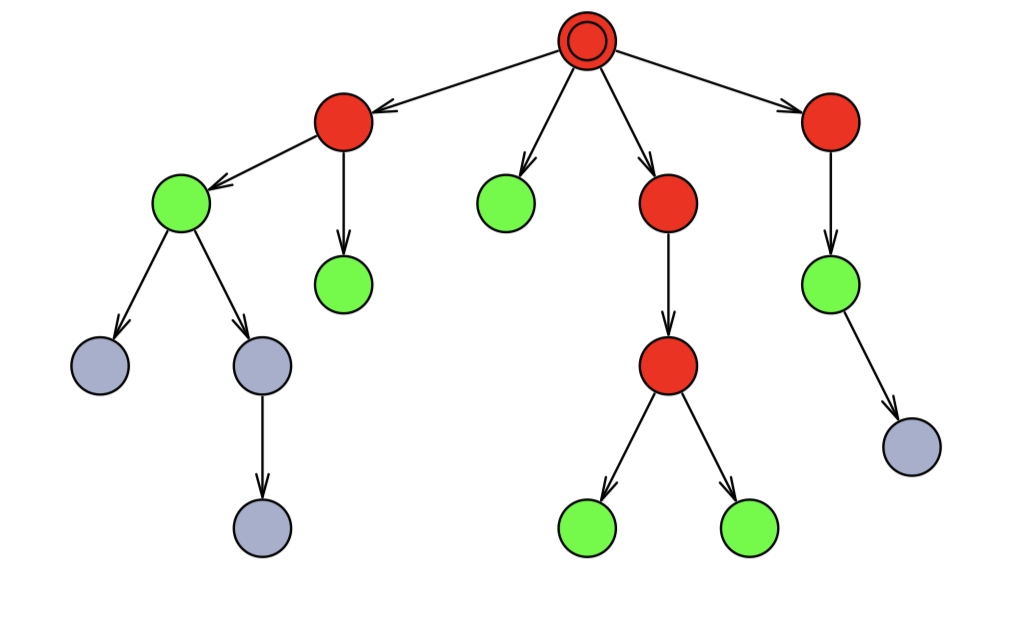
\includegraphics[scale=0.4]{../resources/A(pUq)}
          \caption{Voorbeeld computation tree: operator A(p U q)}
          \label{fig:apug}
        \end{figure}

      \subsubsection{E(p U q)}
        Er is een pad waar geldt 'p U q'.
        \begin{figure}[h]
          \centering
          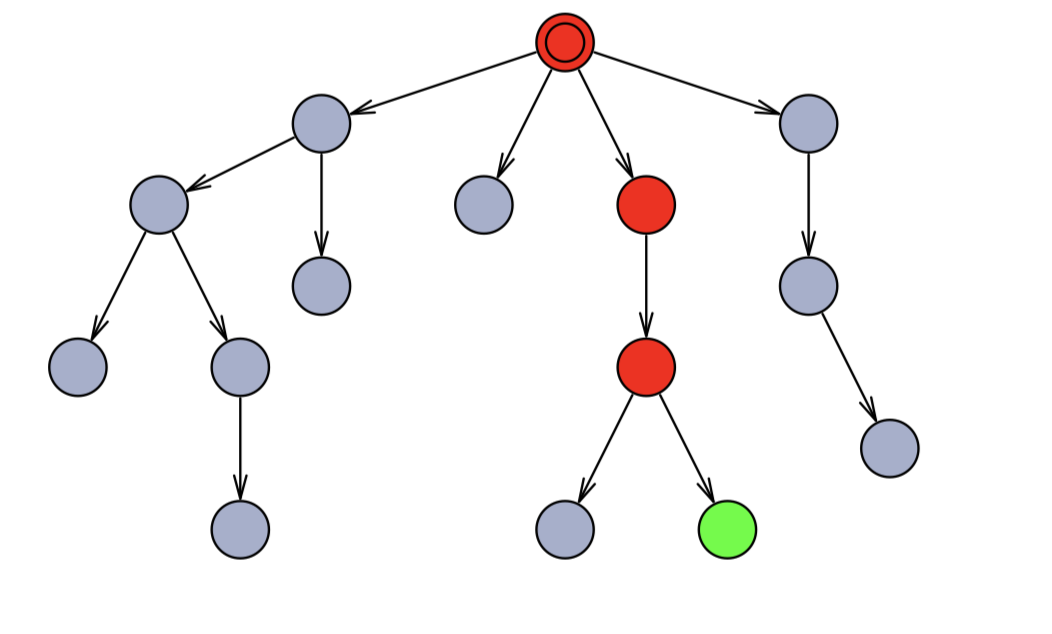
\includegraphics[scale=0.4]{../resources/E(pUq)}
          \caption{Voorbeeld computation tree: operator E(p U q)}
          \label{fig:epug}
        \end{figure}



  \subsection{Operator: p R q}
    \begin{itemize}
      \item 'p' Release 'q'
      \item Uitspraak 'p' is waar voor de states in het pad, totdat 'q' waar is
      \item Er is wel een moment (en state) in de transitie van 'p' naar 'q' waarin beide uitspraken waar zijn
      \item 'q' blijft niet noodzakelijk waar na de transitie
      \item 'p R q' geldt ook als 'q' waar is (vanuit logica)
    \end{itemize}

      \subsubsection{A(p R q)}
        In elk pad geldt 'p R q'.
        \begin{figure}[h]
          \centering
          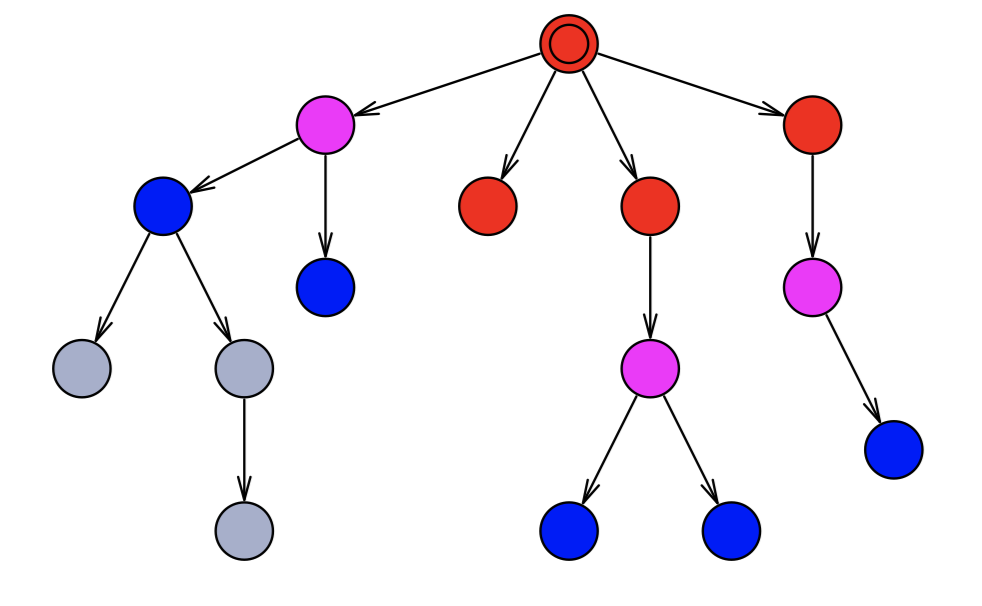
\includegraphics[scale=0.4]{../resources/A(pRq)}
          \caption{Voorbeeld computation tree: operator A(p R q)}
          \label{fig:aprq}
        \end{figure}


      \subsubsection{E(p R q)}
        Er is een pad waar geldt 'p R q'.
        \begin{figure}[h]
          \centering
          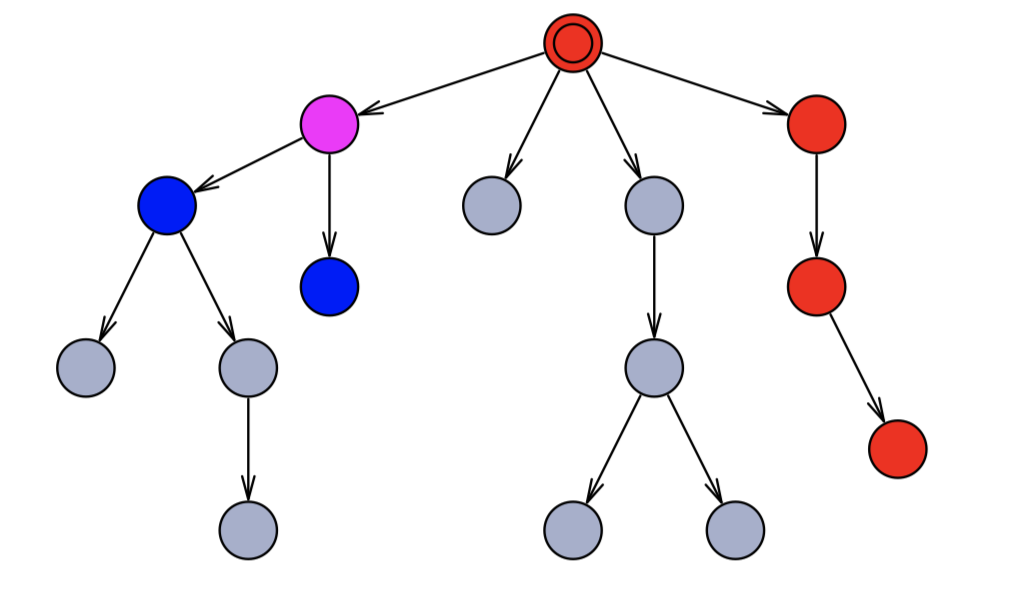
\includegraphics[scale=0.4]{../resources/E(pRq)}
          \caption{Voorbeeld computation tree: operator E(p R q)}
          \label{fig:eprq}
        \end{figure}


  \subsection{Fairness}
    In CTL kunnen ook combinaties van operatoren gebruikt worden. Een veelvoorkomende combinatie is 'AG(AF(p))', wat ook wel liveness wordt genoemd. Oftewel: 'In elke state op elk pad moet AF(p) gelden (in alle de paden na die state komt een state waar p geldt uiteindelijk voor)'.

  \subsection{Liveness}
    Een andere veelvoorkomende combinatie van operatoren is eigenlijk een generalisatie op Fairness: 'AG(p -> AF(q))'. Oftewel: 'als er een state is waar p geldt, dan zal uiteindelijk na die state in alle paden uiteindelijk een state komen waar q geldt'. Liveness heeft zelfs zijn eigen operator: $\rightsquigarrow$.


\newpage

  \newpage
  \bibliography{../resources/references}
  \bibliographystyle{plain}

\end{document}
